% Setting up document structure
\documentclass[a4paper,12pt]{article}
\usepackage[utf8]{vietnam}
\usepackage{amsmath}
\usepackage{amsfonts}
\usepackage{geometry}
\usepackage{parskip}
\usepackage{enumitem}
\usepackage{hyperref}
\usepackage{graphicx}
\usepackage{caption}
\usepackage{xcolor}
\usepackage{tocloft}
\usepackage{titling}
\usepackage{minted}
\usepackage{tikz}
\usepackage{fourier-orns}
\usepackage{fancyhdr}

\renewcommand{\footrule}{%
\vspace{-8pt}\hrulefill
\raisebox{-2.1pt}{\quad\decofourleft\decotwo\decofourright\quad}\hrulefill}

\renewcommand{\headrulewidth}{0pt}
% Set lại vị trí của số trang
\setlength{\headwidth}{\dimexpr\paperwidth-4cm\relax}

% Configuring page margins
\geometry{a4paper, margin=1in}

% Setting up font
\usepackage{times}

% Customizing table of contents
\renewcommand{\cftsecleader}{\cftdotfill{\cftdotsep}}
\setlength{\cftsecindent}{0em}
\setlength{\cftsubsecindent}{2em}

\begin{document}

\pagestyle{fancy}
\fancyhf{}
\fancyhead[R]{\thepage}
% Footer
\fancyfoot[LO]{PGS.TS. Đỗ Văn Nhơn}
\fancyfoot[RO]{Học viên: Lê Hồng Hiển}

% Creating title page
\begin{titlepage}
    \thispagestyle{empty}
    \newgeometry{left=2.75cm, right=2cm, top=0cm, bottom=0cm}
    \begin{tikzpicture}[remember picture, overlay]
        \node[anchor=center] at ([xshift=0.5cm]current page.center) {
\includegraphics[width=\dimexpr\paperwidth-2.5cm\relax,height=\dimexpr\paperheight-2cm\relax]{../images/decorators/cover.png}};
    \end{tikzpicture}
    \vspace*{3cm}
    \begin{center}
        {\bfseries\scshape\LARGE trường đại học công nghệ thông tin \\ khoa khoa học máy tính \par}
        \vspace{1cm}

        % logo
        \begin{center}
            
\includegraphics[width=0.3\textwidth]{../images/decorators/logo.jpg}
        \end{center}

        \vspace{1cm}
        {\bfseries\scshape\Large báo cáo môn học \\ thuật toán và phương pháp giải quyết vấn đề \par}
        \vspace{1cm}
        
        {\huge\bfseries Tìm Đường Đi Tối Ưu cho Xe Buýt tại TP. Hồ Chí Minh Dựa trên Thuật Toán A* và Heuristics \par}
        
        \vspace{2cm}
        {\bfseries\large Học viên: Lê Hồng Hiển - 210101006 \par}
        \vspace{0.5cm}
        {\bfseries\large Giảng viên: PGS.TS. ĐỖ VĂN NHƠN \par}
        \vspace{4cm}
        {\bfseries\itshape\large TP. Hồ Chí Minh, Tháng 6 năm 2025 \par}
    \end{center}
    \restoregeometry
\end{titlepage}

% Adding table of contents
\newpage
% Lời mở đầu
\begin{center}
\section*{Lời mở đầu}
\end{center}
Trong bối cảnh đô thị hóa nhanh chóng tại các thành phố lớn như TP. Hồ Chí Minh, nhu cầu tối ưu hóa giao thông công cộng, đặc biệt là hệ thống xe buýt, ngày càng trở nên cấp thiết. Việc tìm kiếm đường đi tối ưu cho xe buýt không chỉ giúp giảm thời gian di chuyển mà còn góp phần nâng cao hiệu quả sử dụng phương tiện công cộng, giảm ùn tắc giao thông và tiết kiệm chi phí cho người dân. Các bài toán định tuyến giao thông như tìm đường đi ngắn nhất thường có độ phức tạp cao, đặc biệt khi phải xử lý nhiều tuyến xe và các ràng buộc như thời gian chờ, khoảng cách, hay chuyển tuyến. Thuật toán heuristics, với khả năng tìm giải pháp gần tối ưu trong thời gian hợp lý, đã trở thành một công cụ mạnh mẽ để giải quyết các bài toán này.

Báo cáo này trình bày kết quả của dự án phát triển một chương trình tìm đường đi tối ưu cho xe buýt tại TP. Hồ Chí Minh, sử dụng thuật toán A* kết hợp với hàm heuristic dựa trên khoảng cách địa lý. Dự án tập trung vào việc xây dựng một thuật toán có khả năng xử lý dữ liệu từ nhiều tuyến xe buýt khác nhau, với thông tin trạm được cung cấp trước. Ứng dụng được viết bằng Python để xây dựng đồ thị các trạm xe buýt, tính toán thời gian di chuyển dựa trên khoảng cách Haversine, và tối ưu hóa đường đi từ điểm xuất phát và điểm đến được chọn từ trang web. Báo cáo sẽ trình bày chi tiết các bước từ phân tích dữ liệu, thiết kế thuật toán, đến triển khai và đánh giá kết quả, đồng thời thảo luận các thách thức và đề xuất cải tiến cho hệ thống.

Trong quá trình thực hiện, tôi xin gửi lời cảm ơn chân thành đến giáo viên hướng dẫn PGS.TS. Đỗ Văn Nhơn, người đã tận tình hướng dẫn và hỗ trợ tôi trong việc hoàn thành dự án này. Dù đã nỗ lực hết sức, báo cáo không thể tránh khỏi những thiếu sót. Tôi rất mong nhận được những ý kiến đóng góp quý báu từ thầy cô và các bạn để hoàn thiện hơn nội dung và phương pháp thực hiện.

\newpage
\tableofcontents

\newpage
% Starting main content
\section{Cơ sở lý thuyết}

\subsection{Bài toán tìm đường đi trong giao thông công cộng}

\subsubsection{Giới thiệu bài toán}
Trong bối cảnh đô thị hóa và mật độ dân số ngày càng tăng tại các thành phố lớn như TP. Hồ Chí Minh, hệ thống giao thông công cộng, đặc biệt là xe buýt, đóng vai trò quan trọng trong việc đáp ứng nhu cầu di chuyển của người dân. Tuy nhiên, việc lựa chọn đường đi tối ưu khi sử dụng xe buýt thường gặp nhiều khó khăn do sự phức tạp của mạng lưới tuyến xe, bao gồm nhiều trạm dừng, tuyến đường khác nhau, và các ràng buộc như thời gian chờ, khoảng cách di chuyển, hoặc số lần chuyển tuyến. Bài toán tìm đường đi trong giao thông công cộng được định nghĩa là việc xác định một lộ trình từ điểm xuất phát (ví dụ: Chợ Bến Thành) đến điểm đích (ví dụ: Đại học Quốc gia TP.HCM) sao cho tổng thời gian di chuyển là ngắn nhất, đồng thời đảm bảo tính khả thi về mặt thực tế.

Bài toán này thuộc lớp các bài toán tìm đường đi ngắn nhất (shortest path problem) trong lý thuyết đồ thị, nhưng có thêm các đặc điểm đặc thù của hệ thống giao thông công cộng, bao gồm:

\begin{itemize}
    \item \textbf{Đa tuyến}: Một trạm có thể thuộc nhiều tuyến xe buýt, dẫn đến nhiều lựa chọn lộ trình.
    \item \textbf{Chuyển tuyến}: Người dùng có thể phải chuyển từ tuyến này sang tuyến khác tại các trạm chung, kèm theo thời gian chờ.
    \item \textbf{Ràng buộc thời gian}: Thời gian di chuyển phụ thuộc vào lịch trình xe, khoảng cách giữa các trạm, và các yếu tố như kẹt xe.
    \item \textbf{Dữ liệu địa lý}: Vị trí các trạm được biểu diễn bằng tọa độ địa lý (kinh độ và vĩ độ), đòi hỏi phương pháp tính toán khoảng cách phù hợp.
\end{itemize}

\subsubsection{Tầm quan trọng của bài toán}

Việc giải quyết bài toán tìm đường đi trong giao thông công cộng mang lại nhiều lợi ích thiết thực:

\begin{itemize}
    \item \textbf{Giảm thời gian di chuyển}: Giúp người dân tiết kiệm thời gian, tăng cường hiệu quả sử dụng phương tiện công cộng.
    \item \textbf{Tăng cường sử dụng xe buýt}: Một hệ thống tra cứu lộ trình tối ưu sẽ khuyến khích người dân sử dụng xe buýt thay vì phương tiện cá nhân, góp phần giảm ùn tắc giao thông và ô nhiễm môi trường.
    \item \textbf{Hỗ trợ quy hoạch đô thị}: Cung cấp dữ liệu phân tích cho các nhà quản lý giao thông để tối ưu hóa mạng
\end{itemize}

Tại TP. Hồ Chí Minh, với mạng lưới xe buýt gồm hàng trăm tuyến và hàng nghìn trạm dừng, bài toán này càng trở nên quan trọng nhưng cũng đầy thách thức do quy mô lớn và tính phức tạp của dữ liệu.

\subsubsection{Mô hình hóa bài toán}

Để giải quyết bài toán, hệ thống xe buýt được mô hình hóa dưới dạng một \textbf{đồ thị có trọng số} (weighted graph), trong đó:

\begin{itemize}
    \item \textbf{Đỉnh (vertices)}: Đại diện cho các trạm xe buýt, mỗi trạm được xác định bởi mã trạm (stationId), tên trạm (stationName), và tọa độ địa lý (lat, lng).
    \item \textbf{Cạnh (edges)}: Đại diện cho các kết nối giữa hai trạm liên tiếp trên cùng một tuyến xe buýt hoặc giữa các trạm chuyển tuyến. Trọng số của cạnh thường là thời gian di chuyển, được tính dựa trên khoảng cách địa lý hoặc lịch trình thực tế.
    \item \textbf{Trọng số}: Thời gian di chuyển giữa hai trạm, có thể bao gồm:
    \begin{itemize}
        \item Thời gian xe chạy, ước lượng từ khoảng cách Haversine và tốc độ trung bình (ví dụ: 30 km/h).
        \item Thời gian chờ khi chuyển tuyến (ví dụ: 5 phút).
    \end{itemize}
    \item \textbf{Đầu vào}:
    \begin{itemize}
        \item Danh sách các tuyến xe buýt, mỗi tuyến chứa thông tin trạm và trình tự (stationOrder).
        \item Điểm xuất phát và điểm đích, thường là tọa độ địa lý hoặc tên địa điểm (Chợ Bến Thành, Đại học Quốc gia TP.HCM).
    \end{itemize}
    \item \textbf{Đầu ra}:
    \begin{itemize}
        \item Một chuỗi các trạm cần đi qua, các tuyến xe sử dụng, và tổng thời gian ước tính.
        \item Ví dụ: Đi tuyến 01 từ trạm A đến trạm B, chuyển sang tuyến 50 tại trạm B, đến trạm C.
    \end{itemize}
\end{itemize}

\subsubsection{Thách thức bài toán}

Bài toán tìm đường đi trong giao thông công cộng đối mặt với một số thách thức:
\begin{itemize}
    \item \textbf{Quy mô dữ liệu lớn}: Hệ thống xe buýt TP. Hồ Chí Minh có hàng nghìn trạm và hàng trăm tuyến, dẫn đến đồ thị với số lượng đỉnh và cạnh lớn.
    \item \textbf{Tính động}: Thời gian di chuyển thay đổi theo giờ cao điểm, kẹt xe, hoặc lịch trình xe buýt.
    \item \textbf{Chuyển tuyến phức tạp}: Việc xác định các trạm chuyển tuyến hợp lý đòi hỏi tính toán khoảng cách địa lý và thời gian chờ, đồng thời tối ưu hóa số lần chuyển tuyến.
\end{itemize}
Do độ phức tạp tính toán của bài toán, các thuật toán tìm kiếm chính xác như Dijkstra hoặc Bellman-Ford có thể không hiệu quả khi đồ thị lớn. Thay vào đó, thuật toán dựa trên heuristic, như A* \cite{cormen2009}, là một lựa chọn phù hợp để tìm giải pháp gần tối ưu trong thời gian hợp lý.

\subsubsection{Phạm vi nghiên cứu}

Trong báo cáo này, bài toán được giới hạn ở việc tìm đường đi tối ưu từ Chợ Bến Thành đến Đại học Quốc gia TP.HCM, sử dụng dữ liệu tuyến xe buýt dưới dạng file JSON. Các giả định được áp dụng bao gồm:
\begin{itemize}
    \item Tốc độ xe buýt trung bình là 30 km/h.
    \item Thời gian chờ khi chuyển tuyến là 5 phút.
    \item Khoảng cách tối đa để chuyển tuyến giữa hai trạm là 500m.
    \item Dữ liệu tuyến bao gồm thông tin trạm (stationId, Name, Lat, Lng) và trình tự tuyến (stationOrder).
\end{itemize}
Phạm vi này giúp đơn giản hóa bài toán để tập trung vào việc triển khai thuật toán A* \cite{cormen2009} và đánh giá hiệu quả, đồng thời vẫn đảm bảo tính thực tiễn trong bối cảnh TP. Hồ Chí Minh.

\subsection{Thuật toán A*}
Thuật toán A* \cite{cormen2009} là một thuật toán tìm kiếm đường đi tối ưu trong đồ thị, được giới thiệu bởi Hart, Nilsson và Raphael vào năm 1968 [1]. Đây là một thuật toán heuristic, kết hợp giữa tìm kiếm theo chiều rộng (breadth-first search) và tìm kiếm theo chi phí thấp nhất (uniform-cost search), nhằm đảm bảo tìm được đường đi ngắn nhất với hiệu suất cao.

\subsubsection{Nguyên lý hoạt động}

A* \cite{cormen2009} sử dụng một hàm chi phí tổng quát để đánh giá các đỉnh trong đồ thị: $f(n) = g(n) + h(n)$, trong đó:
\begin{itemize}
    \item $g(n)$ Chi phí thực tế từ đỉnh xuất phát đến đỉnh hiện tại $n$. Trong bài toán xe buýt, $g(n)$ được tính dựa trên thời gian di chuyển giữa các trạm, bao gồm cả thời gian chờ khi chuyển tuyến.
    \item $h(n)$ Chi phí ước lượng (heuristic) từ đỉnh hiện tại $n$ đến đích. Hàm heuristic phải thỏa mãn hai điều kiện:
    \begin{itemize}
        \item \textbf{Admissible}: $h(n) \leq h^n$, trong đó $h^n$ là chi phí thực tế từ $n$ đến đích.
        \item \textbf{Monotonic (hoặc consistent)}: Đối với mọi cạnh từ $n$ đến $m$, $h(n) \leq h(m) + c(n, m)$, với $c(n, m)$ là chi phí cạnh từ $n$ đến $m$.
    \end{itemize}
\end{itemize}

A* \cite{cormen2009} sử dụng hàng đợi ưu tiên (priority queue) để luôn ưu tiên mở rộng các đỉnh có giá trị $f(n)$ nhỏ nhất, đảm bảo tìm được đường đi tối ưu với số lần duyệt ít hơn so với các thuật toán như Dijkstra.

\subsubsection{Ưu điểm và hạn chế}

\begin{itemize}
    \item \textbf{Ưu điểm}:
    \begin{itemize}
        \item Đảm bảo tìm được đường đi ngắn nhất nếu heuristic thỏa mãn điều kiện admissible và monotonic.
        \item Hiệu quả hơn Dijkstra khi có heuristic tốt, vì giảm số đỉnh cần duyệt.
    \end{itemize}
    \item \textbf{Hạn chế}:
    \begin{itemize}
        \item Hiệu suất phụ thuộc vào chất lượng của hàm heuristic.
        \item Yêu cầu bộ nhớ lớn hơn so với các thuật toán tìm kiếm đơn giản như tìm kiếm sâu (DFS).
    \end{itemize}
\end{itemize}
Trong bài toán tìm đường đi xe buýt, A* được chọn vì khả năng xử lý đồ thị lớn với nhiều tuyến xe buýt và các trạm chuyển tuyến, đồng thời tận dụng heuristic để giảm thời gian \cite{delling2009}.

\subsection{Hàm Heuristic}
Hàm heuristic đóng vai trò quan trọng trong thuật toán A*, giúp định hướng tìm kiếm đến đích nhanh hơn. Trong bài toán này, chúng tôi sử dụng \textbf{khoảng cách Haversine} giữa hai trạm để ước lượng thời gian di chuyển từ trạm hiện tại đến đích \cite{hart1968} \cite{elmihoub2006}.

\subsubsection{Công thức tính khoảng cách Haversine}
Công thức Haversine tính khoảng cách giữa hai điểm trên bề mặt Trái Đất dựa trên kinh độ (longitude) và vĩ độ (latitude):
\[
a = \sin^2\left(\frac{\Delta \phi}{2}\right) + \cos(\phi_1) \cdot \cos(\phi_2) \cdot \sin^2\left(\frac{\Delta \lambda}{2}\right)
\]
\[
c = 2 \cdot \arctan2\left(\sqrt{a}, \sqrt{1-a}\right)
\]
\[
d = R \cdot c
\]

Trong đó:
\begin{itemize}
    \item $\phi_1, \phi_2$: Vĩ độ của hai điểm (radian).
    \item $\lambda_1, \lambda_2$: Kinh độ của hai điểm (radian).
    \item $R$: Bán kính Trái Đất (khoảng 6371 km).
    \item $d$: Khoảng cách tính bằng kilômét.
\end{itemize}
Thời gian ước lượng được tính bằng cách nhân khoảng cách  với một hệ số tốc độ (giả định 30 km/h, tương đương 2 phút/km).

\subsubsection{Tính chất của heuristic}

\begin{itemize}
    \item \textbf{Admissible}: Khoảng cách Haversine luôn nhỏ hơn hoặc bằng khoảng cách thực tế trên tuyến xe buýt, vì xe buýt không thể di chuyển theo đường thẳng mà phải theo lộ trình cố định.
    \item \textbf{Monotonic}: Vì khoảng cách Haversine giữa các điểm gần nhau giảm dần khi tiến gần đến đích, heuristic này đảm bảo tính nhất quán.
    \item \textbf{Lý do chọn}: Haversine đơn giản, dễ tính toán, và phù hợp với bài toán địa lý, đồng thời tận dụng dữ liệu kinh độ/vĩ độ có sẵn trong file JSON.
\end{itemize}

\subsection{Hàm Heuristic áp dụng trong bài toán}

\subsubsection{Mô hình hóa bài toán thành đồ thị}

Bài toán được mô hình hóa dưới dạng một đồ thị có hướng:
\begin{itemize}
    \item \textbf{Đỉnh}: Các trạm xe buýt (được xác định bởi stationId, lat, lng).
    \item \textbf{Cạnh}:
    \begin{itemize}
        \item Kết nối các trạm liên tiếp trong cùng một tuyến xe buýt (dựa trên stationOrder).
        \item Kết nối các trạm chuyển tuyến (khoảng cách < 500m) với thời gian chờ bổ sung (giả định 5 phút).
    \end{itemize}
    \item \textbf{Trọng số}: Thời gian di chuyển giữa các trạm, tính bằng khoảng cách Haversine nhân với hệ số tốc độ.
\end{itemize}

\subsubsection{Cấu trúc dữ liệu đầu vào}

Dữ liệu được cung cấp dưới dạng file JSON, mỗi file đại diện cho một tuyến xe buýt với các trường chính \cite{busplan}:
\begin{itemize}
    \item \texttt{routeNo}: Mã số tuyến (ví dụ: "01").
    \item \texttt{routeName}: Tên tuyến (ví dụ: "Bến Thành - Bến Xe buýt Chợ Lớn").
    \item \texttt{stations}: Danh sách trạm với các thông tin như \texttt{stationId}, \texttt{stationName}, \texttt{lat}, \texttt{lng}, \texttt{stationOrder}.
\end{itemize}
Dữ liệu này được xử lý để:
\begin{itemize}
    \item Tạo danh sách trạm và tuyến từ dữ liệu JSON.
    \item Xây dựng đồ thị với các cạnh dựa trên thứ tự trạm và chuyển tuyến.
    \item Tính toán thời gian di chuyển và thời gian chờ.
\end{itemize}

\subsubsection{Ví dụ minh họa}

Với dữ liệu tuyến 01 (Bến Thành - Chợ Lớn) và tuyến giả định 50 (Bến Thành - ĐH Quốc gia), đồ thị bao gồm:
\begin{itemize}
    \item Các trạm liên tiếp trong tuyến 01 (ví dụ: từ \texttt{stationId: 7266} đến \texttt{stationId: 7693}).
    \item Chuyển tuyến từ trạm chung (ví dụ: \texttt{stationId: 7266} thuộc cả tuyến 01 và 50).
    \item Heuristic từ mỗi trạm đến Đại học Quốc gia được tính dựa trên khoảng cách Haversine.
\end{itemize}

\newpage
\section{Mô tả yêu cầu}

Chương này trình bày quá trình phân tích yêu cầu bài toán tìm đường đi tối ưu cho xe buýt tại TP. Hồ Chí Minh, phân tích dữ liệu đầu vào, thiết kế thuật toán dựa trên thuật toán A* và heuristic, cũng như mô tả các công cụ và môi trường triển khai. Mục tiêu là xây dựng một hệ thống generic, có khả năng xử lý dữ liệu từ nhiều tuyến xe buýt, đảm bảo tìm được đường đi ngắn nhất về thời gian.

\subsection{Mô tả yêu cầu}

Bài toán tìm đường đi tối ưu cho xe buýt được xác định với các yêu cầu cụ thể như sau:

\subsubsection{Input}
\begin{itemize}
    \item \textbf{Điểm xuất phát}: Chọn từ danh sách. Ví dụ: Chợ Bến Thành (tọa độ: 10.7755, 106.6983).
    \item \textbf{Điểm đến}: Chọn từ danh sách. Ví dụ: Đại học Quốc gia TP.HCM (tọa độ: 10.874479, 106.807659).
    \item \textbf{Dữ liệu tuyến xe}: Danh sách các file JSON, mỗi file đại diện cho một tuyến xe buýt, chứa thông tin về:
    \begin{itemize}
        \item Mã tuyến (\texttt{routeNo})
        \item Tên tuyến (\texttt{routeName})
        \item Danh sách trạm (\texttt{stations}) với các thuộc tính:
        \begin{itemize}
            \item Mã trạm (\texttt{stationId})
            \item Tên trạm (\texttt{stationName})
            \item Tọa độ (\texttt{lat}, \texttt{lng})
            \item Thứ tự trạm (\texttt{stationOrder})
        \end{itemize}
    \end{itemize}
\end{itemize}

\subsubsection{Output}
\begin{itemize}
    \item Danh sách các trạm cần đi qua, bao gồm các tuyến xe buýt sử dụng và điểm chuyển tuyến (nếu có).
    \item Thời gian ước tính cho toàn bộ hành trình (tính bằng phút).
\end{itemize}

\subsubsection{Ràng buộc}
\begin{itemize}
    \item Hệ thống phải hỗ trợ chuyển tuyến giữa các tuyến xe buýt khác nhau.
    \item Thời gian di chuyển giữa các trạm được tính dựa trên khoảng cách địa lý và tốc độ giả định.
    \item Thời gian chờ khi chuyển tuyến cần được xem xét.
    \item Hệ thống phải dễ dàng mở rộng khi thêm dữ liệu tuyến mới.
\end{itemize}

\subsubsection{Mục tiêu}
Mục tiêu chính là tìm đường đi có tổng thời gian ngắn nhất, đồng thời đảm bảo tính chính xác và hiệu quả tính toán khi xử lý nhiều tuyến xe buýt.


\subsection{Phân tích dữ liệu}
Dữ liệu đầu vào đóng vai trò quan trọng trong việc xây dựng hệ thống. Dựa trên các file JSON đầu vào, cấu trúc dữ liệu được phân tích như sau:

\subsubsection{Cấu trúc file JSON}
\begin{itemize}
    \item \textbf{routeNo}: Mã tuyến (ví dụ: "01")
    \item \textbf{routeName}: Tên tuyến (ví dụ: "Bến Thành - Bến Xe buýt Chợ Lớn")
    \item \textbf{stations}: Danh sách các trạm, mỗi trạm bao gồm:
    \begin{itemize}
        \item \texttt{stationId}: Mã định danh duy nhất của trạm (ví dụ: 7266 cho "Trạm Trung chuyển trên đường Hàm Nghi")
        \item \texttt{stationName}: Tên trạm (ví dụ: "Chợ Kim Biên")
        \item \texttt{lat, lng}: Tọa độ địa lý của trạm (ví dụ: 10.751253, 106.652565)
        \item \texttt{stationOrder}: Thứ tự trạm trên tuyến (từ 0 đến số trạm cuối)
        \item \texttt{stationDirection}: Chiều đi (0) hoặc về (1), giúp xác định lộ trình
    \end{itemize}
\end{itemize}

\subsubsection{Giả định}
\begin{itemize}
    \item Tốc độ xe buýt trung bình là 30 km/h, tương đương 0.5 km/phút, để tính thời gian di chuyển giữa các trạm
    \item Thời gian chờ chuyển tuyến là 5 phút
    \item Chỉ sử dụng các trạm có \texttt{stationDirection = 0} (chiều đi) để đơn giản hóa đồ thị
\end{itemize}

\subsection{Thiết kế thuật toán}
Dữ liệu được đọc từ các file JSON và chuyển thành danh sách các đối tượng \texttt{BusStop} (trạm) và map \texttt{routes} (lộ trình từng tuyến), phục vụ cho việc xây dựng đồ thị. Hệ thống được thiết kế với các bước chính sau:

\begin{enumerate}
    \item \textbf{Đọc và xử lý dữ liệu}
    \begin{itemize}
        \item Hàm \texttt{load\_routes} đọc danh sách file JSON, tạo danh sách các trạm (\texttt{BusStop}) với thuộc tính \texttt{stationId}, \texttt{name}, \texttt{lat}, \texttt{lng}, và \texttt{route\_no}.
        \item Tạo map \texttt{routes} ánh xạ mã tuyến (\texttt{routeNo}) đến danh sách \texttt{stationId} theo thứ tự (\texttt{stationOrder}).
    \end{itemize}
    
    \item \textbf{Xây dựng đồ thị}
    \begin{itemize}
        \item Hàm \texttt{build\_graph} thực hiện:
        \begin{itemize}
            \item \textbf{Kết nối trong tuyến}: Với mỗi tuyến, kết nối các trạm liên tiếp (theo \texttt{stationOrder}) bằng cạnh có trọng số là thời gian di chuyển, tính bằng công thức: $\text{thời gian} = \text{khoảng cách Haversine} \times 2$. Khoảng cách Haversine được tính dựa trên tọa độ (\texttt{lat}, \texttt{lng}) của hai trạm.
            \item \textbf{Kết nối chuyển tuyến}: Nếu hai trạm thuộc các tuyến khác nhau và cách nhau dưới 500m, tạo cạnh với thời gian: $\text{thời gian} = \text{khoảng cách Haversine} \times 2 + 5$. Trong đó, 5 phút là thời gian chờ giả định.
        \end{itemize}
        \item Kết quả là một đồ thị có hướng, với các đỉnh là \texttt{stationId} và các cạnh bao gồm (\texttt{neighbor\_id}, \texttt{time}, \texttt{route\_info}).
    \end{itemize}
    
    \item \textbf{Tìm trạm gần nhất}
    \begin{itemize}
        \item Hàm \texttt{find\_nearest\_stop} tìm trạm có khoảng cách Haversine nhỏ nhất đến tọa độ của điểm xuất phát và điểm đích.
        \item Kết quả trả về \texttt{stationId} của trạm xuất phát và đích.
    \end{itemize}
    
    \item \textbf{Áp dụng thuật toán A*}
    \begin{itemize}
        \item Hàm \texttt{a\_star} sử dụng thuật toán A* để tìm đường đi ngắn nhất:
        \begin{itemize}
            \item \textbf{Hàng đợi ưu tiên}: Lưu trữ các trạng thái (\texttt{f}, \texttt{g}, \texttt{node}, \texttt{path}, \texttt{route\_path}), với:
            \begin{itemize}
                \item $f = g + h$: Tổng chi phí ước lượng
                \item $g$: Thời gian từ xuất phát đến trạm hiện tại
                \item $h$: Heuristic, ước lượng thời gian từ trạm hiện tại đến đích (dựa trên khoảng cách Haversine nhân với 2)
            \end{itemize}
            \item \textbf{Heuristic}: $h = \text{khoảng cách Haversine} \times 2$. Hàm này là admissible vì không bao giờ ước lượng quá cao thời gian thực tế.
            \item \textbf{Xử lý chuyển tuyến}: Lưu thông tin tuyến (\texttt{route\_info}) để xác định khi nào cần chuyển tuyến.
        \end{itemize}
        \item Kết quả trả về danh sách \texttt{path} (các trạm), \texttt{route\_path} (các tuyến), và \texttt{total\_time}.
    \end{itemize}
    
    \item \textbf{Trích xuất kết quả}
    \begin{itemize}
        \item Chuyển danh sách \texttt{stationId} thành tên trạm và hiển thị lộ trình, bao gồm:
        \begin{itemize}
            \item Các trạm đi qua
            \item Tuyến xe sử dụng
            \item Điểm chuyển tuyến (nếu có)
            \item Tổng thời gian ước tính
        \end{itemize}
    \end{itemize}
\end{enumerate}

\subsection{Mã nguồn chính}

Dưới đây là các hàm xử lý chính của thuật toán:

\begin{minted}[breaklines,fontsize=\footnotesize]{python}
def heuristic(stop_id, goal_id, stop_dict):
    """Hàm heuristic"""
    stop1 = stop_dict[stop_id]
    stop2 = stop_dict[goal_id]
    distance = haversine(stop1.lat, stop1.lng, stop2.lat, stop2.lng)
    return distance * 2  # Thời gian ước lượng (phút)

def a_star(start_id, goal_id, graph, stop_dict):
    """Thuật toán A* tìm đường đi ngắn nhất"""
    queue = [(0, 0, start_id, [], [])]  # (f, g, node, path, routes)
    visited = set()
    
    while queue:
        f, g, node, path, route_path = heapq.heappop(queue)
        state = (node, tuple(route_path[-1:]))
        if state in visited:
            continue
        visited.add(state)
        
        path = path + [node]
        
        if node == goal_id:
            return path, route_path, g
        
        for neighbor, cost, route_info in graph.get(node, []):
            if (neighbor, route_info) not in visited:
                new_g = g + cost
                h = heuristic(neighbor, goal_id, stop_dict)
                f = new_g + h
                new_route_path = route_path + [route_info]
                heapq.heappush(queue, (f, new_g, neighbor, path, new_route_path))
    
    return None, None, float('inf')
\end{minted}

\subsection{Công cụ}

Hệ thống được triển khai với các công cụ và môi trường sau:

\begin{itemize}
    \item \textbf{Ngôn ngữ lập trình}: Python 3 \cite{python2025}, do tính phổ biến, dễ sử dụng, và có nhiều thư viện hỗ trợ.
    
    \item \textbf{Thư viện}:
    \begin{itemize}
        \item \texttt{heapq}: Cung cấp hàng đợi ưu tiên cho thuật toán A*.
        \item \texttt{json}: Đọc và xử lý file JSON.
        \item \texttt{math}: Hỗ trợ tính toán khoảng cách Haversine (các hàm sin, cos, radians, v.v.).
        \item \texttt{flask}: Xây dựng API Backend cho website.
    \end{itemize}
    
    \item \textbf{Dữ liệu mẫu}: Các file JSON chứa thông tin các tuyến xe buýt TP.HCM.
    
    \item \textbf{Tính mở rộng}: Hệ thống được thiết kế để dễ dàng mở rộng bằng cách thêm các file JSON mới vào danh sách đầu vào, không cần thay đổi mã nguồn chính.
\end{itemize}

\newpage
\section{Triển khai và Kết quả}
\subsection{Triển khai chương trình}
\subsubsection{Môi trường phát triển}

Hệ thống được triển khai trên nền tảng Python 3 với các thư viện hỗ trợ chuyên biệt cho việc xử lý thuật toán tìm đường và quản lý dữ liệu. Môi trường phát triển được thiết lập với các công cụ sau:

\begin{itemize}
    \item \texttt{heapq}: Hỗ trợ hàng đợi ưu tiên cho thuật toán A*.
    \item \texttt{math}: Cung cấp các hàm toán học để tính khoảng cách Haversine.
    \item \texttt{json}: Đọc và xử lý dữ liệu tuyến xe buýt từ file JSON.
\end{itemize}

Mã nguồn được viết bằng Python 3, đảm bảo tính đơn giản và dễ mở rộng để xử lý dữ liệu từ nhiều tuyến xe buýt. Toàn bộ mã nguồn được cung cấp trong Phụ lục A.

\subsubsection{Các thành phần chính của chương trình}

Chương trình bao gồm các hàm chính sau:

\begin{itemize}
    \item \texttt{haversine(lat1, lon1, lat2, lon2)}: Tính khoảng cách địa lý giữa hai điểm dựa trên công thức Haversine. Khoảng cách (km) được chuyển thành thời gian (phút) với tốc độ giả định 30 km/h.
    
    \item \texttt{load\_routes(route\_files)}: Đọc dữ liệu từ các file JSON, tạo danh sách các trạm (BusStop) và ánh xạ các tuyến (routes).
    
    \item \texttt{build\_graph(stops, routes)}: Xây dựng đồ thị:
    \begin{itemize}
        \item Kết nối các trạm liên tiếp trong cùng tuyến, với chi phí là thời gian di chuyển.
        \item Kết nối các trạm chuyển tuyến (khoảng cách < 500m) với chi phí bao gồm thời gian chờ (5 phút).
    \end{itemize}
    
    \item \texttt{heuristic(stop\_id, goal\_id, stop\_dict)}: Tính chi phí ước lượng từ trạm hiện tại đến đích dựa trên khoảng cách Haversine.
    
    \item \texttt{a\_star(start\_id, goal\_id, graph, stop\_dict)}: Thực hiện thuật toán A* để tìm đường đi ngắn nhất về thời gian.
    
    \item \texttt{find\_nearest\_stop(target\_lat, target\_lng, stops)}: Tìm trạm gần nhất với điểm xuất phát hoặc đích dựa trên tọa độ.
\end{itemize}

Mã nguồn được tổ chức thành ba file chính: \texttt{bus\_route\_finder.py} (thuật toán tìm đường), \texttt{bus\_route\_api.py} (API Backend), và \texttt{bus\_route\_ui.html} (giao diện người dùng). Hệ thống dễ dàng chạy trên máy tính có Python3 với dữ liệu đầu vào là danh sách các chuỗi JSON hoặc file JSON.

\subsubsection{Dữ liệu đầu vào}

Dữ liệu được sử dụng bao gồm 10 file JSON đại diện cho 10 tuyến xe thực tế có số hiệu từ 1 đến 10 đang hoạt động tại TP.HCM. Dữ liệu được thu thập từ phần mềm BusMap \cite{busmap}, một phần mềm lớn về đặt xe buýt tại Việt Nam đang hoạt động.

Mỗi tuyến xe buýt sẽ bao gồm các thông tin:
\begin{itemize}
    \item \textbf{Số hiệu tuyến buýt}: Ví dụ: xe buýt số 1, xe buýt số 10,...
    \item \textbf{Tên tuyến xe buýt}: Ví dụ: Bến Thành - Bến Xe buýt Chợ Lớn
    \item \textbf{Danh sách trạm}: Bao gồm tên trạm, id, kinh độ, vĩ độ, địa chỉ,...
    \item \textbf{Các thông tin khác}: Giá vé, giá vé tháng, loại tuyến, công ty, thời gian hoạt động,...
\end{itemize}

\subsection{Kết quả thực nghiệm}
\subsubsection{Kịch bản thử nghiệm}

Chương trình được thử nghiệm với kịch bản tìm đường đi tối ưu từ Bến xe buýt Chợ Lớn đến Bến xe buýt ĐH Quốc gia TPHCM (mới). Các bước thực hiện:

\begin{itemize}
    \item \textbf{Điểm bắt đầu}: Bến xe buýt Chợ Lớn (GA HKXB CHO LON, đường Lê Quang Sung, Quận 5).
    \item \textbf{Điểm kết thúc}: Bến xe buýt ĐH Quốc gia TPHCM (mới) (Trạm nạp CNG ĐH Quốc gia, đường Nguyễn Hiền, TP. Thủ Đức - KV3).
    \item \textbf{Thuật toán}: Áp dụng thuật toán A* để tìm đường đi ngắn nhất về thời gian, có thể bao gồm chuyển tuyến.
\end{itemize}

\subsubsection{Kết quả thực nghiệm}

Kết quả chạy chương trình cho thấy đường đi tối ưu như sau:

\textbf{Đường đi:}
\begin{itemize}
    \item \textbf{Lên xe tuyến 05} tại: Bến xe buýt Chợ Lớn (GA HKXB CHO LON, đường Lê Quang Sung, Quận 5)
    
    \item \textbf{Đi qua các trạm:}
    \begin{itemize}
        \item Tạ Uyên (79, đường Tạ Uyên, Quận 5)
        \item Tạ Uyên ((516)816, đường Nguyễn Chí Thanh, Quận 11)
        \item Chợ Thiếc (698, đường Nguyễn Chí Thanh, Quận 11)
        \item Bệnh viện Răng Hàm Mặt (598, đường Nguyễn Chí Thanh, Quận 11)
        \item Nhà máy Bia Sài Gòn (Đối diện nhà máy bia Sài Gòn, đường Nguyễn Chí Thanh, Quận 10)
        \item Ngã tư Ngô Quyền (440, đường Nguyễn Chí Thanh, Quận 10)
        \item Nguyễn Tiểu La (292, đường Nguyễn Chí Thanh, Quận 10)
        \item Trường CĐ Sư phạm TW thành phố (184, đường Nguyễn Chí Thanh, Quận 10)
        \item Ngã tư Trần Nhân Tông (126, đường Hùng Vương, Quận 10)
        \item Ngã tư Lê Hồng Phong (88, đường Hùng Vương, Quận 10)
        \item Ngã tư Trần Bình Trọng (Kế số 2, đường Hùng Vương, Quận 10)
        \item Công viên Âu Lạc (Đối diện số 1, đường Hùng Vương, Quận 10)
        \item Nhà sách Minh Khai (488, đường Nguyễn Thị Minh Khai, Quận 3)
        \item Trung ương Hội Chữ thập đỏ TP (464 - 466, đường Nguyễn Thị Minh Khai, Quận 3)
        \item Bệnh viện Từ Dũ (436, đường Nguyễn Thị Minh Khai, Quận 3)
        \item Tôn Thất Tùng (414, đường Nguyễn Thị Minh Khai, Quận 3)
        \item Cách Mạng tháng 8 (284, đường Nguyễn Thị Minh Khai, Quận 3)
        \item Nguyễn Thị Minh Khai (17, đường Bà Huyện Thanh Quan, Quận 3)
        \item Đại học Mở thành phố HCM (62, đường Võ Văn Tần, Quận 3)
        \item Trần Quốc Thảo (44, đường Võ Văn Tần, Quận 3)
        \item Bảo tàng chứng tích chiến tranh (28, đường Võ Văn Tần, Quận 3)
        \item Sân Phan Đình Phùng (8, đường Võ Văn Tần, Quận 3)
        \item Hồ Con Rùa (24 - 26, đường Trần Cao Vân, Quận 3)
        \item Phùng Khắc Khoan (2 - 4, đường Phùng Khắc Khoan, Quận 1)
        \item Nhà thờ Mạc Ti Nho (16A, đường Nguyễn Thị Minh Khai, Quận 1)
        \item Đài truyền hình (Đối diện 9, đường Nguyễn Thị Minh Khai, Quận 1)
        \item Thảo Cầm Viên (2A, đường Nguyễn Thị Minh Khai, Quận 1)
        \item Nhà thờ Thị Nghè (79, đường Xô Viết Nghệ Tĩnh, Quận Bình Thạnh)
        \item Ngã ba Nguyễn Cửu Vân (151, đường Xô Viết Nghệ Tĩnh, Quận Bình Thạnh)
        \item Trường Tiểu học Hồng Hà (153, đường Xô Viết Nghệ Tĩnh, Quận Bình Thạnh)
        \item Trường trung học Gia Định (221, đường Xô Viết Nghệ Tĩnh, Quận Bình Thạnh)
        \item Chợ Hàng Xanh (39, đường Bạch Đằng, Quận Bình Thạnh)
        \item Trạm xăng dầu (17, đường Đinh Bộ Lĩnh, Quận Bình Thạnh)
        \item Cầu Đinh Bộ Lĩnh (85, đường Đinh Bộ Lĩnh, Quận Bình Thạnh)
        \item Ngã Tư Chu Văn An (183, đường Đinh Bộ Lĩnh, Quận Bình Thạnh)
        \item Ngã Tư Nguyễn Xí (291-293, đường Đinh Bộ Lĩnh, Quận Bình Thạnh)
    \end{itemize}
    
    \item \textbf{Chuyển tuyến} tại: Cổng vào-Bến xe Miền Đông (78/3, đường Đinh Bộ Lĩnh, Quận Bình Thạnh) \textbf{(từ tuyến 05 sang tuyến 08)}
    
    \item \textbf{Đi qua các trạm:}
    \begin{itemize}
        \item Ngã tư Bình Triệu (599, đường Phạm Văn Đồng, TP. Thủ Đức - KV3)
        \item Đường số 20 (218, đường Phạm Văn Đồng, TP. Thủ Đức - KV3)
        \item Cá sấu Hoa Cà (Trụ chiếu sáng B194, đường Phạm Văn Đồng, TP. Thủ Đức - KV3)
        \item Chùa An Lạc (Ngã tư Hiệp Bình - PVĐ, đường Phạm Văn Đồng, TP. Thủ Đức - KV3)
        \item Nút giao Linh Đông -PVĐ (Trụ chiếu sáng A226, đường Phạm Văn Đồng, TP. Thủ Đức - KV3)
        \item Trường Cao đẳng Vinatex (403, đường Kha Vạn Cân, TP. Thủ Đức - KV3)
        \item Trạm xăng 27-7 (459 (Đối diện 624), đường Kha Vạn Cân, TP. Thủ Đức - KV3)
        \item Công an Phường Linh Đông (525, đường Kha Vạn Cân, TP. Thủ Đức - KV3)
        \item Trạm Cầu ngang (569, đường Kha Vạn Cân, TP. Thủ Đức - KV3)
        \item Chợ Thủ Đức (20-21, đường Lê Văn Ninh, TP. Thủ Đức - KV3)
    \end{itemize}
    
    \item \textbf{Chuyển tuyến} tại: Ngã ba Chương Dương (Đối diện 100, đường Võ Văn Ngân, TP. Thủ Đức - KV3) \textbf{(từ tuyến 08 sang tuyến 06)}
    
    \item \textbf{Đi qua các trạm:}
    \begin{itemize}
        \item Cao đẳng xây dựng 2 (233 (253), đường Võ Văn Ngân, TP. Thủ Đức - KV3)
        \item Nhà thiếu nhi Thủ Đức (Nhà thiếu nhi, đường Võ Văn Ngân, TP. Thủ Đức - KV3)
        \item Siêu thị Nguyễn Kim (307 (312), đường Võ Văn Ngân, TP. Thủ Đức - KV3)
        \item Trường Đại học Sư phạm Kỹ thuật (1, đường Võ Văn Ngân, TP. Thủ Đức - KV3)
        \item Công ty Cocacola (Công ty Cocacola, đường Xa Lộ Hà Nội, TP. Thủ Đức - KV3)
        \item Xa Lộ Hà Nội (Đối diện Khu Công Nghệ Cao Q.9, đường Xa Lộ Hà Nội, TP. Thủ Đức - KV3)
    \end{itemize}

    \item \textbf{Chuyển tuyến} tại: Khu Công nghệ cao Q9 (Đối diện Khu công nghệ cao, đường Xa Lộ Hà Nội, TP. Thủ Đức - KV3) \textbf{(từ tuyến 06 sang tuyến 08)}
    
    \item \textbf{Đi qua các trạm:}
    \begin{itemize}
        \item Câu vượt Trạm 2 (Câu vượt Trạm 2, đường Quốc lộ 1, TP. Thủ Đức - KV3)
        \item Khu DL Suối Tiên (9/29, đường Quốc lộ 1, TP. Thủ Đức - KV3)
        \item Trường giáo dục Quốc phòng (Trường giáo dục Quốc phòng, đường Quốc lộ 1, TP. Thủ Đức - KV3)
        \item Đi qua: Đại học An Ninh Nhân Dân (Nhà máy Tiến Thành, đường Quốc lộ 1, TP. Thủ Đức - KV3)
        \item Chuyển tuyến tại: ĐH Khoa học tự nhiên (đối diện trạm CNG , đường Đường 621, TP. Thủ Đức - KV3) (từ tuyến 08 sang tuyến 10)
    \end{itemize}
    \item \textbf{Xuống xe tại}: Bến xe buýt ĐH Quốc gia TPHCM (mới) (Trạm nạp CNG ĐH Quốc gia, đường Nguyễn Hiền, TP. Thủ Đức - KV3)
\end{itemize}

\textbf{Thời gian ước tính}: 48.45 phút

\subsubsection{Hình ảnh minh họa}
Hình ảnh minh họa các trang web demo, tìm đường đi và kết quả.

\begin{figure}[H]
    \centering
    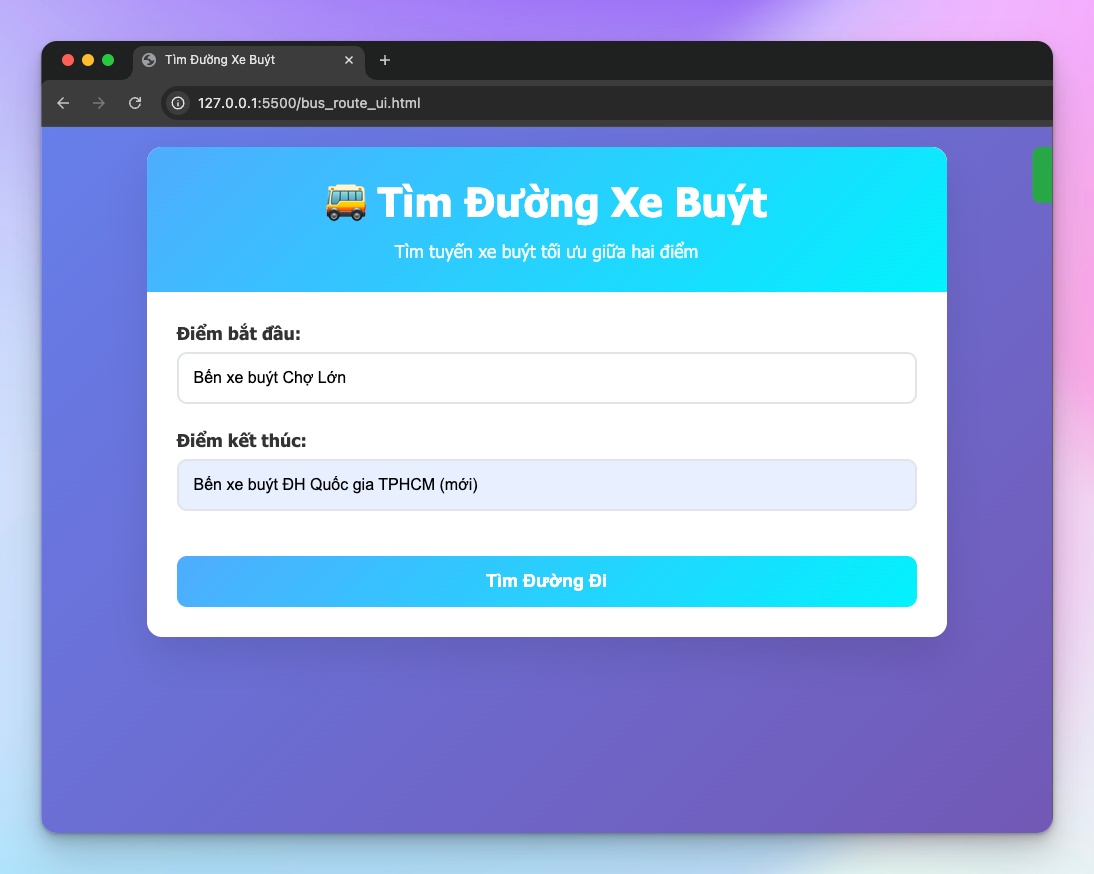
\includegraphics[width=0.9\textwidth]{images/image1.png}
    \caption{Trang web demo}
    \label{fig:demo}
\end{figure}

\begin{figure}[H]
    \centering
    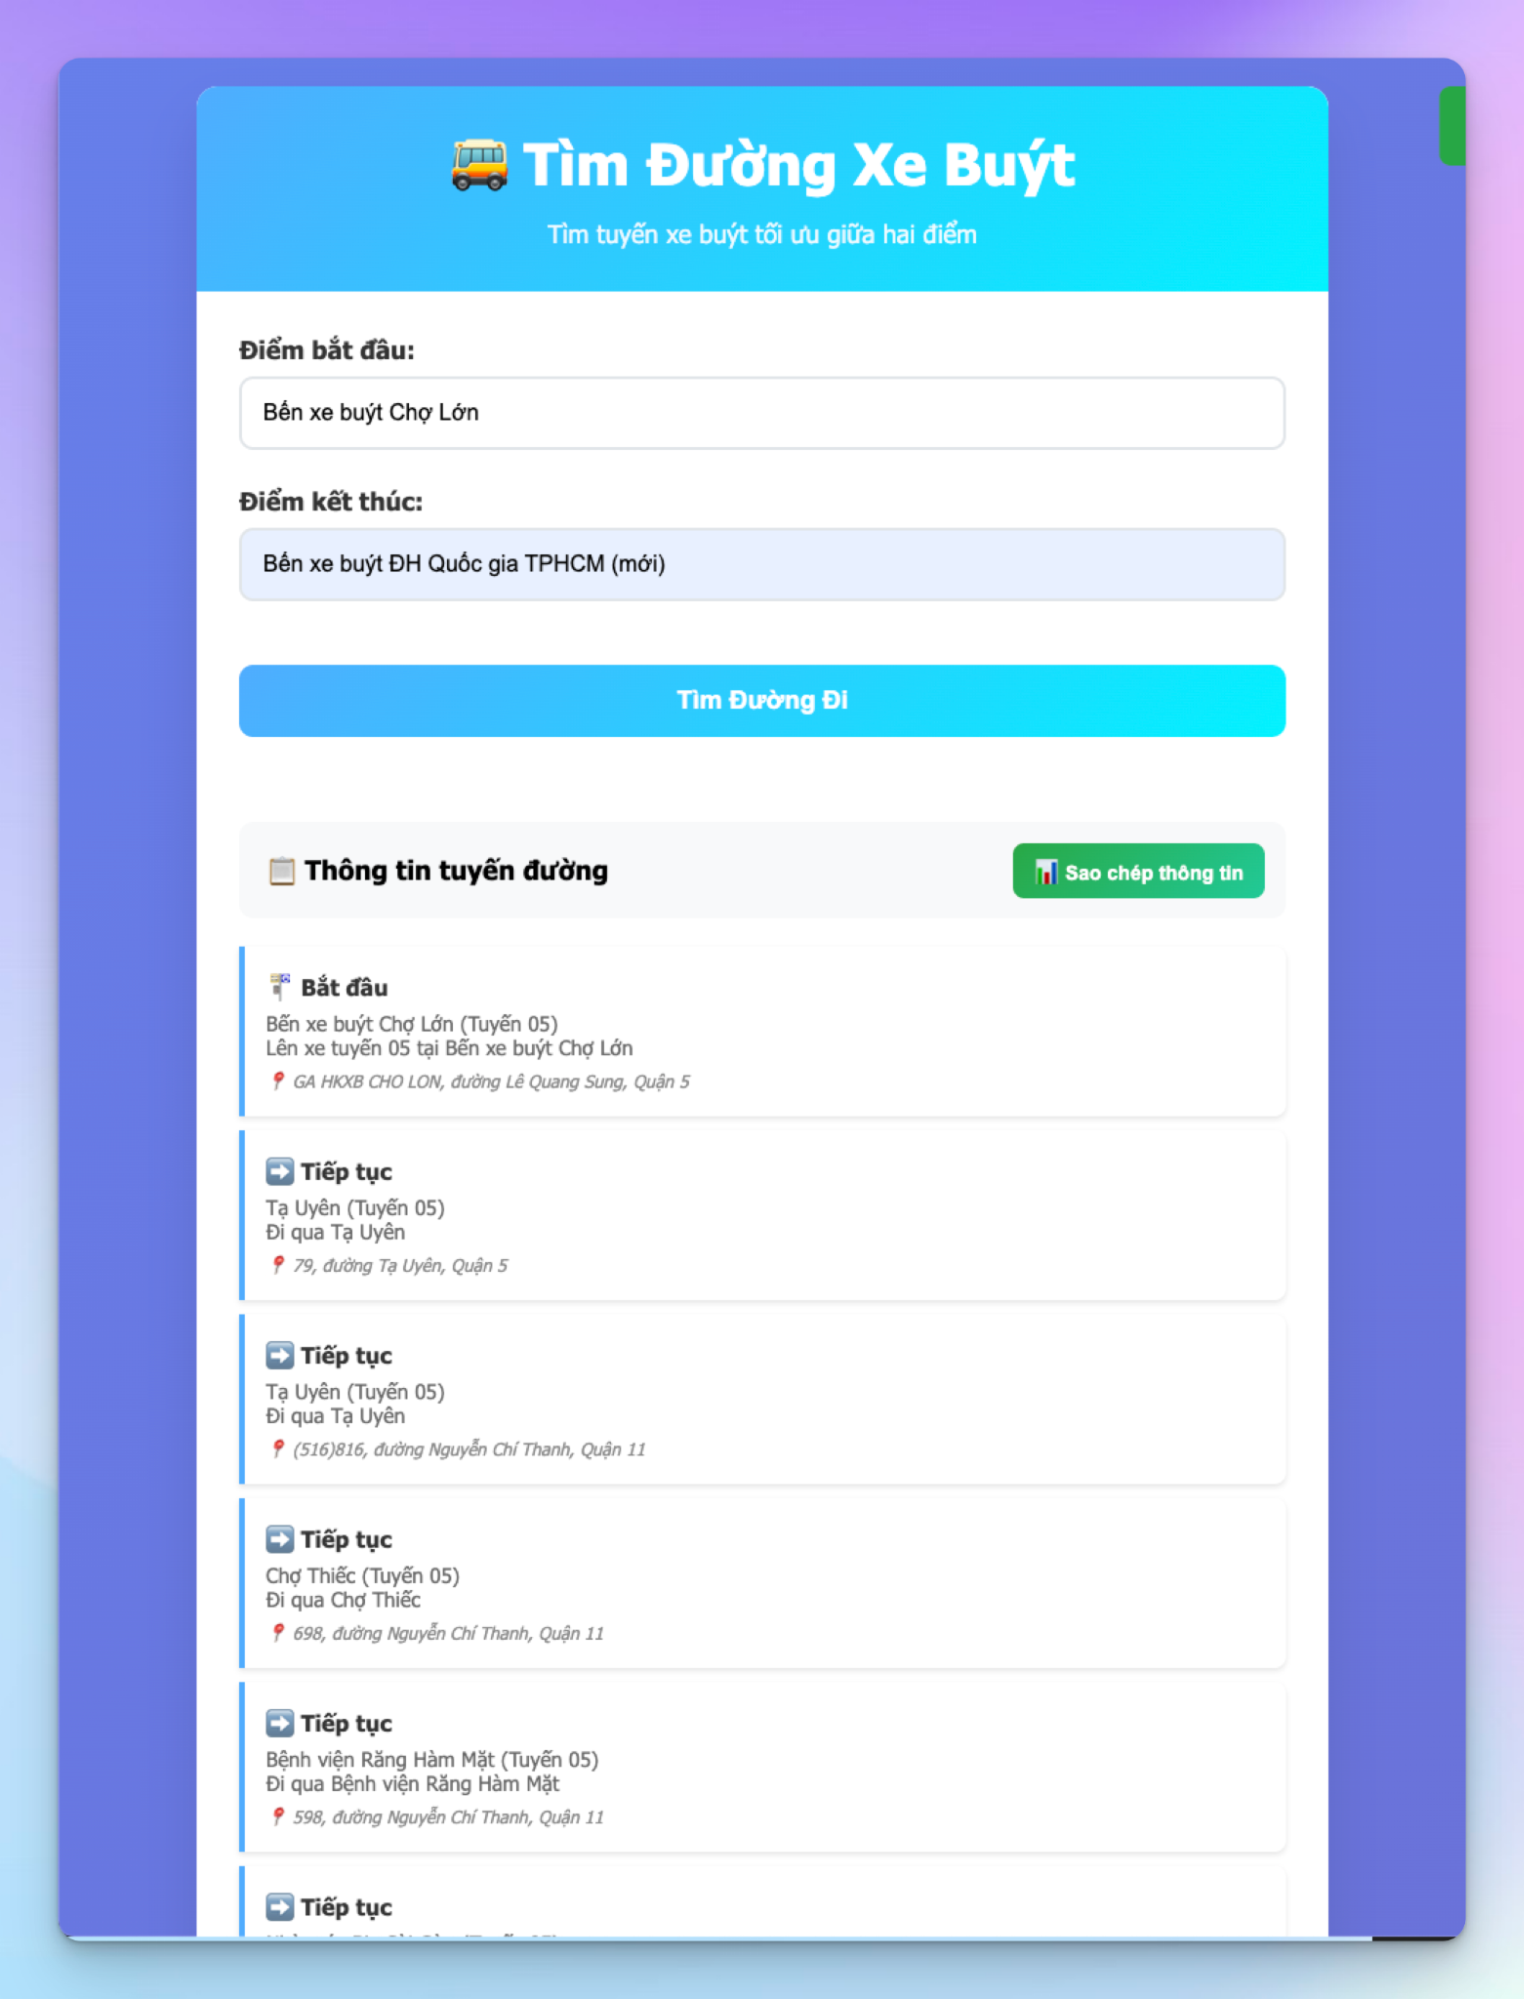
\includegraphics[width=0.9\textwidth]{images/image2.png}
    \caption{Tìm đường đi}
    \label{fig:search}
\end{figure}

\begin{figure}[H]
    \centering
    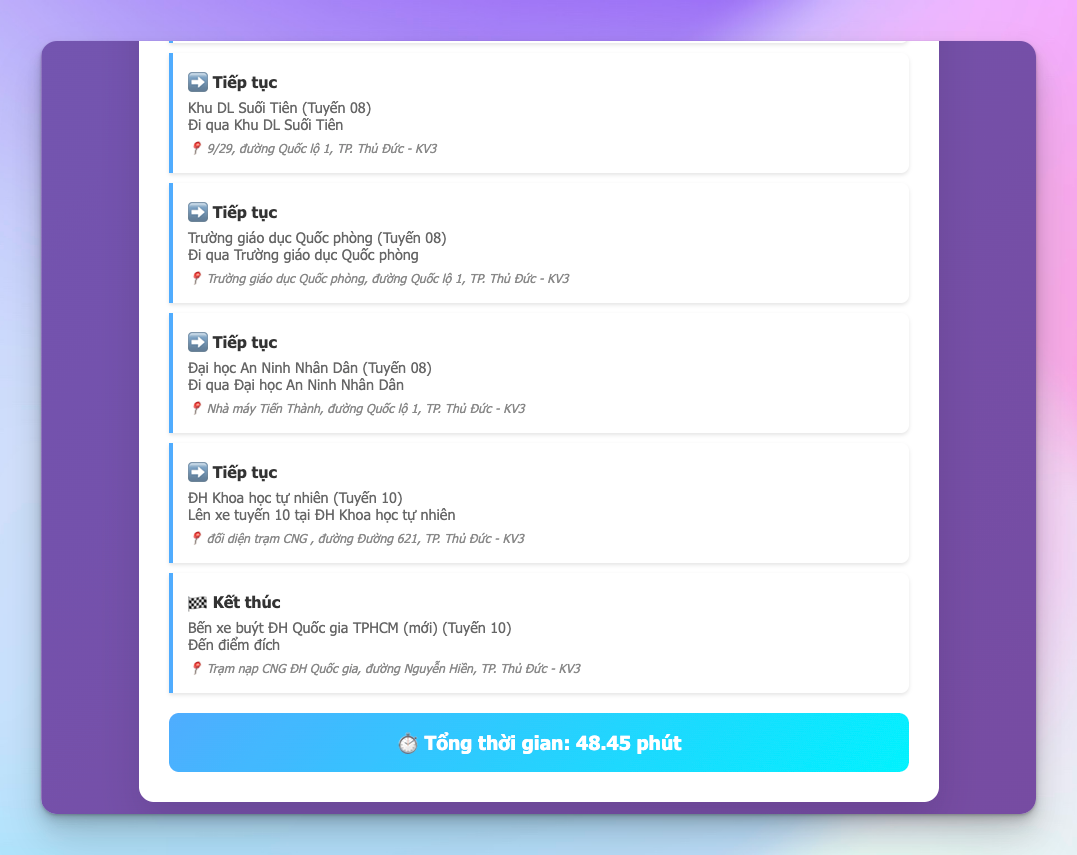
\includegraphics[width=0.9\textwidth]{images/image3.png}
    \caption{Kết quả}
    \label{fig:result}
\end{figure}

\subsubsection{Đánh giá}

\begin{itemize}
    \item \textbf{Độ chính xác}: Đường đi được tìm thấy là hợp lý, yêu cầu chuyển tuyến vài lần. Kết quả phù hợp với mục tiêu tối ưu hóa thời gian di chuyển.
    
    \item \textbf{Hiệu suất}: Thuật toán A* chạy nhanh nhờ heuristic Haversine hiệu quả và đồ thị quy mô nhỏ. Độ phức tạp trung bình là $O(E \log V)$, với $E$ là số cạnh và $V$ là số đỉnh.
    
    \item \textbf{Hạn chế}: 
    \begin{itemize}
        \item Dữ liệu về số tuyến xe buýt còn ít. Cần bổ sung thêm dữ liệu thực tế để đảm bảo tính ứng dụng.
        \item Thời gian di chuyển ước tính dựa trên tốc độ cố định (30 km/h), chưa tính đến các yếu tố như kẹt xe, thời gian dừng trạm, hoặc lịch trình thực tế.
    \end{itemize}
\end{itemize}

\subsection{Thách thức gặp phải}
Trong quá trình triển khai, một số thách thức đã được ghi nhận:

\begin{itemize}
    \item \textbf{Dữ liệu hạn chế}: Chỉ có dữ liệu 10 tuyến xe buýt tuy là dữ liệu thật nhưng còn khá ít. Trong thực tế, cần thu thập dữ liệu đầy đủ từ các tuyến xe buýt TP.HCM (như tuyến 08, 10, 19, 50).
    
    \item \textbf{Giả định đơn giản hóa}:
    \begin{itemize}
        \item Tốc độ xe buýt cố định (30 km/h) không phản ánh điều kiện giao thông thực tế.
        \item Thời gian chờ chuyển tuyến (5 phút) là giá trị ước lượng, chưa dựa trên lịch trình thực tế từ timeTableIn/timeTableOut.
    \end{itemize}
    
    \item \textbf{Xử lý đồ thị phức tạp}: Khi số lượng tuyến và trạm tăng, việc xây dựng đồ thị và tính toán khoảng cách Haversine có thể trở nên tốn kém hơn. Cần tối ưu hóa thêm cho dữ liệu lớn.
    
    \item \textbf{Triển khai thực tế}: Chương trình hiện chạy trên Colab, chưa được tích hợp vào ứng dụng người dùng cuối (như web hoặc mobile app).
\end{itemize}

Để khắc phục, dự án có thể cải tiến bằng cách:
\begin{itemize}
    \item Thu thập dữ liệu đầy đủ từ BusMap \cite{busmap} hoặc Sở Giao thông Vận tải TP.HCM.
    \item Tích hợp lịch trình thời gian thực hoặc dữ liệu giao thông.
    \item Cập nhật giao diện người dùng để trực quan hóa đường đi.
\end{itemize}

\newpage
\section{Thảo luận và Hướng phát triển}
\subsection{Thảo luận}
\subsubsection{Ưu điểm của phương pháp}

Dự án phát triển hệ thống tìm đường đi tối ưu cho xe buýt tại TP. Hồ Chí Minh sử dụng thuật toán A* với heuristic dựa trên khoảng cách Haversine đã đạt được một số kết quả nhất định. Những ưu điểm chính bao gồm:

\begin{itemize}
    \item \textbf{Hiệu quả tính toán}: Thuật toán A* tận dụng hàm heuristic để giảm không gian tìm kiếm, giúp tìm đường đi ngắn nhất về mặt thời gian một cách nhanh chóng, ngay cả khi đồ thị có số lượng trạm lớn. So với các thuật toán tìm kiếm không sử dụng heuristic như Dijkstra, A* giảm đáng kể thời gian chạy nhờ định hướng tìm kiếm dựa trên ước lượng khoảng cách đến đích.
    
    \item \textbf{Tính generic}: Hệ thống được thiết kế để xử lý dữ liệu từ nhiều file JSON đại diện cho các tuyến xe buýt khác nhau. Chỉ cần cung cấp thêm file dữ liệu với cấu trúc tương tự, chương trình có thể mở rộng để hỗ trợ toàn bộ hệ thống xe buýt TP. Hồ Chí Minh mà không cần sửa đổi mã nguồn.
    
    \item \textbf{Dễ triển khai}: Việc sử dụng Python và có thể chạy trực tiếp trên Google Colab giúp chương trình dễ dàng được chạy trên nhiều nền tảng mà không yêu cầu cấu hình phần cứng phức tạp. Thư viện chuẩn như heapq và math đảm bảo tính ổn định và khả năng tái sử dụng.
    
    \item \textbf{Khả năng xử lý chuyển tuyến}: Hệ thống tự động xác định các trạm chuyển tuyến dựa trên khoảng cách địa lý (dưới 500m), cho phép mô phỏng thực tế quá trình chuyển tuyến của hành khách.
\end{itemize}


\subsubsection{Hạn chế của phương pháp}

Mặc dù đạt được một số kết quả tích cực, hệ thống vẫn tồn tại một số hạn chế cần được xem xét:

\begin{itemize}
    \item \textbf{Dữ liệu hạn chế}: Chỉ có dữ liệu thực tế từ 10 tuyến xe buýt tại TP.HCM. Điều này làm giảm tính thực tiễn của kết quả, vì dữ liệu chưa đủ độ phức tạp, không phản ánh chính xác hệ thống xe buýt thực tế.
    
    \item \textbf{Giả định đơn giản hóa}: Thời gian di chuyển giữa các trạm được tính dựa trên khoảng cách Haversine và tốc độ cố định (30 km/h), không tính đến các yếu tố thực tế như kẹt xe, thời gian dừng trạm, hoặc sự thay đổi tốc độ theo thời điểm trong ngày. Thời gian chờ chuyển tuyến (5 phút) cũng là một ước lượng cố định, không phản ánh tần suất thực tế của các chuyến xe.
    
    \item \textbf{Heuristic đơn giản}: Hàm heuristic hiện tại chỉ dựa trên khoảng cách địa lý, không tích hợp các yếu tố như tần suất xe buýt, thời gian chờ, hoặc số lần chuyển tuyến. Điều này có thể dẫn đến việc chọn đường đi không tối ưu trong một số trường hợp thực tế.
    
    \item \textbf{Khả năng mở rộng hạn chế}: Mặc dù hệ thống có tính generic, việc xử lý dữ liệu lớn (hàng trăm tuyến xe và hàng nghìn trạm) có thể làm tăng thời gian chạy thuật toán, đặc biệt nếu đồ thị trở nên phức tạp hơn.
\end{itemize}

\subsubsection{So sánh với các phương pháp khác}

Để đánh giá hiệu quả của thuật toán A*, có thể so sánh với một số phương pháp khác:

\begin{itemize}
    \item \textbf{Thuật toán Dijkstra}: Dijkstra đảm bảo tìm đường đi ngắn nhất nhưng không sử dụng heuristic, dẫn đến việc khám phá nhiều đỉnh hơn A*. Trong bài toán này, A* vượt trội hơn do giảm không gian tìm kiếm, đặc biệt khi đồ thị có nhiều trạm.
    
    \item \textbf{Tìm kiếm sâu (DFS)}: DFS có thể tìm đường đi nhưng không đảm bảo tối ưu và dễ bị mắc kẹt trong các vòng lặp hoặc đường đi dài không cần thiết. A* khắc phục vấn đề này nhờ hàm heuristic và hàng đợi ưu tiên.
    
    \item \textbf{Các phương pháp meta-heuristic}: Các thuật toán như Genetic Algorithm hoặc Simulated Annealing có thể áp dụng cho bài toán định tuyến xe buýt, nhưng chúng phức tạp hơn và thường không đảm bảo giải pháp tối ưu. A* là lựa chọn phù hợp hơn cho bài toán này do yêu cầu giải pháp nhanh và chính xác.
\end{itemize}


\subsection{Hướng phát triển}

Để nâng cao hiệu quả và tính thực tiễn của hệ thống, một số hướng phát triển sau được đề xuất:

\begin{itemize}
    \item \textbf{Tích hợp dữ liệu thực tế}: Thu thập thêm dữ liệu từ nhiều tuyến xe buýt thực tế tại TP. Hồ Chí Minh hơn nữa, bao gồm thông tin về tần suất xe (timeTableIn, timeTableOut), thời gian dừng trạm, và các yếu tố ảnh hưởng như tình trạng giao thông. Điều này sẽ giúp hệ thống phản ánh chính xác hơn thực tế vận hành.
    
    \item \textbf{Cải tiến hàm heuristic}: Kết hợp thêm các yếu tố vào hàm heuristic, chẳng hạn như tần suất xe buýt, thời gian chờ thực tế tại trạm, hoặc số lần chuyển tuyến tối thiểu. Một heuristic phức tạp hơn có thể được xây dựng bằng cách sử dụng dữ liệu lịch sử về thời gian di chuyển thực tế hoặc dự đoán kẹt xe.
    
    \item \textbf{Tích hợp thời gian thực}: Phát triển hệ thống để kết nối với dữ liệu thời gian thực từ các nguồn như GPS của xe buýt hoặc ứng dụng giao thông công cộng. Điều này cho phép cập nhật thời gian chờ và thời gian di chuyển theo tình hình giao thông thực tế.
    
    \item \textbf{Cải thiện ứng dụng người dùng}: Đối với web thì cập nhật lại giao diện để thân thiện với người dùng hơn, thêm bản đồ minh hoạ để hiển thị nhiều lựa chọn khác nhau, thời gian ước tính, đường đi tối ưu,... Thêm Backend và Database để lưu lại lịch sử di chuyển, các tuyến xe ưa thích hoặc bắn thông báo tới người dùng.
    
    \item \textbf{Tối ưu hóa nhiều tiêu chí}: Ngoài tối ưu hóa thời gian, hệ thống có thể được mở rộng để cân nhắc tối ưu thêm các tiêu chí khác như chi phí vé, số lần chuyển tuyến, hoặc mức độ thoải mái (ví dụ: ưu tiên tuyến xe có điều hòa). Điều này yêu cầu thuật toán A* được điều chỉnh để xử lý bài toán đa mục tiêu.
    
    \item \textbf{Tăng cường hiệu suất}: Đối với dữ liệu lớn, có thể áp dụng các kỹ thuật như chia nhỏ đồ thị thành các cụm trạm theo khu vực địa lý hoặc sử dụng cơ sở dữ liệu đồ thị (như Neo4j) để quản lý và truy vấn hiệu quả hơn.
\end{itemize}

\newpage
\begin{center}
\addcontentsline{toc}{section}{Tổng kết}
\section*{Tổng kết}
\end{center}

Dự án phát triển chương trình tìm đường đi tối ưu cho xe buýt tại TP. Hồ Chí Minh đã đạt được những kết quả đáng ghi nhận. Bằng cách sử dụng thuật toán A* kết hợp với hàm heuristic dựa trên khoảng cách Haversine, chương trình đã thành công trong việc tìm ra đường đi ngắn nhất về mặt thời gian, có khả năng xử lý chuyển tuyến và tích hợp dữ liệu từ các file JSON mô tả các tuyến xe buýt. Việc triển khai code với Python đảm bảo tính dễ tiếp cận và khả năng mở rộng khi có thêm dữ liệu thực tế. Kết quả thực nghiệm cho thấy chương trình có thể tìm đường đi tối ưu với thời gian ước tính khoảng 48.45 phút, đi qua các trạm trung gian và chuyển tuyến một cách hợp lý.

Qua quá trình thực hiện, tôi đã củng cố kiến thức về thuật toán A* và các phương pháp heuristic, đồng thời nắm bắt được cách xử lý dữ liệu thực tế trong các bài toán giao thông. Những thách thức như dữ liệu hạn chế, giả định đơn giản về thời gian di chuyển, và xử lý chuyển tuyến đã giúp tôi hiểu rõ hơn về sự phức tạp của các bài toán định tuyến trong thực tiễn. Bên cạnh đó, việc thiết kế hệ thống generic để xử lý nhiều tuyến xe đã nâng cao kỹ năng lập trình và phân tích vấn đề của tôi.

Trong tương lai, dự án có thể được cải tiến bằng cách tích hợp dữ liệu thực tế từ các tuyến xe buýt khác tại TP. Hồ Chí Minh, bổ sung thời gian chờ thực tế từ lịch trình xe, và xem xét các yếu tố như kẹt xe hay thời gian dừng trạm. Ngoài ra, việc phát triển một ứng dụng di động hoặc web dựa trên thuật toán này sẽ mang lại giá trị thực tiễn cao, giúp người dân dễ dàng tra cứu đường đi xe buýt. Dự án cũng mở ra hướng nghiên cứu áp dụng các thuật toán heuristics khác hoặc kết hợp với học máy để tối ưu hóa thêm các tiêu chí như chi phí hoặc số lần chuyển tuyến.

Mặc dù đã đạt được những kết quả khả quan, dự án vẫn còn những hạn chế cần khắc phục. Tôi hy vọng báo cáo này sẽ nhận được những ý kiến đóng góp quý báu từ thầy cô và các bạn để hoàn thiện hơn, đồng thời tạo nền tảng cho các nghiên cứu sâu hơn trong lĩnh vực tối ưu hóa giao thông công cộng.


\newpage
\begin{center}
\addcontentsline{toc}{section}{Tài liệu tham khảo}
\section*{Tài liệu tham khảo}
\end{center}
\vspace{-2em}
\renewcommand{\refname}{}
\begin{thebibliography}{99}

\bibitem{cormen2009}
Cormen, T. H., Leiserson, C. E., Rivest, R. L., \& Stein, C. (2009). \textit{Introduction to Algorithms} (3rd ed.). MIT Press.

\bibitem{hart1968}
Hart, P. E., Nilsson, N. J., \& Raphael, B. (1968). A Formal Basis for the Heuristic Determination of Minimum Cost Paths. \textit{IEEE Transactions on Systems Science and Cybernetics}, 4(2), 100-107.

\bibitem{busplan}
Azavea. (n.d.). \textit{BusPlan: Open Source School Bus Routing Optimization}. GitHub. Truy cập tại: \url{https://github.com/azavea/bus-plan}.

\bibitem{delling2009}
Delling, D., Sanders, P., Schultes, D., \& Wagner, D. (2009). Engineering Route Planning Algorithms. \textit{Algorithmics of Large and Complex Networks}, 117-139.

\bibitem{opentripplanner}
OpenTripPlanner. (n.d.). \textit{OpenTripPlanner Documentation}. Truy cập tại: \url{https://docs.opentripplanner.org/en/latest/}.

\bibitem{busmap}
BusMap.vn. (n.d.). \textit{Dữ liệu tuyến xe buýt TP. Hồ Chí Minh}. Truy cập tại: \url{https://busmap.vn/}.

\bibitem{python2025}
Python Software Foundation. (2025). \textit{Python Documentation}. Truy cập tại: \url{https://docs.python.org/3/}.

\bibitem{elmihoub2006}
El-Mihoub, T. A., Hopgood, A. A., Nolle, L., \& Battersby, A. (2006). Hybrid Genetic Algorithms: A Review. \textit{Engineering Letters}, 13(2), 11-15.

\end{thebibliography}

\end{document}